%%%%%%%%%%%%%%%%%%%%%%%%%%%%%%%%%%%%%%%%%%%%%%%%
% E.Pinault-Bigeard - e.pinault-bigeard@upsti.fr
% http://s2i.pinault-bigeard.com
% CC BY-NC-SA 2.0 FR - http://creativecommons.org/licenses/by-nc-sa/2.0/fr/
%%%%%%%%%%%%%%%%%%%%%%%%%%%%%%%%%%%%%%%%%%%%%%%%
\documentclass[11pt,english]{article}

%%%%%%%%%%%%%%%%%%%%%%%%%%%%%%%%%%%%%%%%%%%%%%%%
% Package UPSTI_Document
%%%%%%%%%%%%%%%%%%%%%%%%%%%%%%%%%%%%%%%%%%%%%%%%
%%%%%%%%%%%%%%%%%%%%%%%%%%%%%%%%%%%%%%%%%%%%%%%%
% Package UPSTI_Document
%%%%%%%%%%%%%%%%%%%%%%%%%%%%%%%%%%%%%%%%%%%%%%%%
\usepackage{subcaption}
%\usepackage[usenames, svgnames, dvipsnames]{xcolor}
\RequirePackage{UPSTI_Document}
%\RequirePackage{multicol}
%\usepackage{pgfplots}
%\definecolor{darkspringgreen}{rgb}{0.09, 0.45, 0.27}
%
% \newcommandx*{\dessinRepereFigGeo}[5][1=\vx{},2=\vy{},3=\vz{},4=,5=0]
% 	{
% 		\draw [->,very thick] (0,0) -- (1,0) ;
% 		\draw [->,very thick] (0,0) -- (0,1) ;
%     \fill[white] (0,0) circle (0.13);
%     \draw [->,very thick] (0,0) circle (0.13);
%     \ifnumequal{#5}{0} {% z vers nous
%       \fill[black] (0,0) circle (0.03);
%       \draw [->,thick] (0,0) circle (0.04);
%     }{% z vers la feuille
%   		\begin{scope} [rotate=45]
%   			\draw [-,thick] (0,-0.12) -- (0,0.12) ;
%   			\draw [-,thick] (-0.12,0) -- (0.12,0) ;
%   		\end{scope}
%     }
% 		\draw [anchor=north west] (1.1,0) node {${#1}$};
% 		\draw [anchor=south west] (0,1.1) node {${#2}$};
% 		\draw [anchor=north east] (-0.1,0) node {${#3}$};
% 		\draw [anchor=north west] (-0.1,-0.1) node {${#4}$};
% 	}

	% \usepackage{array}
	% \newcolumntype{L}[1]{>{\raggedright\let\newline\\\arraybackslash\hspace{0pt}}m{#1}}
	% \newcolumntype{C}[1]{>{\centering\let\newline\\\arraybackslash\hspace{0pt}}m{#1}}
	% \newcolumntype{R}[1]{>{\raggedleft\let\newline\\\arraybackslash\hspace{0pt}}m{#1}}

\RequirePackage{dirtree}
%
\RequirePackage[cache=false]{minted}
% \RequirePackage{tcolorbox}
% \RequirePackage{etoolbox}
% \BeforeBeginEnvironment{minted}{\begin{tcolorbox}}%
% \AfterEndEnvironment{minted}{\end{tcolorbox}}%

% %
\RequirePackage[abs]{overpic}
\RequirePackage{fp}
\RequirePackage{siunitx}
\RequirePackage{multicol}

\RequirePackage{float}
\newfloat{codeFloat}{htbp}{lop}
\floatname{codeFloat}{Programme}
%
% %
\RequirePackage{xparse}
\ExplSyntaxOn
\NewDocumentCommand {\RoundingUpFunction} { m }
 {
  \fp_eval:n { ceil(#1) }
 }
\ExplSyntaxOff

\ExplSyntaxOn
\NewDocumentCommand {\RoundingDownFunction} { m }
 {
  \fp_eval:n { floor(#1) }
 }
\ExplSyntaxOff


%---------------------------------%
% Paramètres du package
%---------------------------------%

% Version du document (pour la compilation)
% 1: Document prof
% 2: Document élève
% 3: Document à publier
\newcommand{\UPSTIidVersionDocument}{2}


% Variante
%\newcommand{\UPSTIvariante}{2}

% Classe
% 1: PTSI				6: PSI*			11: TSI2		16: Spé
% 2: PT	(par défaut)	7: MPSI			12: ATS
% 3: PT*				8: MP			13: PC
% 4: PCSI				9: MP*			14: PC*
% 5: PSI				10: TSI1		15: Sup
%\newcommand{\UPSTIidClasse}{2}

% Affichage personnalisé de la classe
\newcommand{\UPSTIclasse}{TUK}
\newcommand{\UPSTIvariante}{8}
% Matière
% 1: S2I (par défaut)    2: IPT     3: TIPE
% 6: Vie au lycée
\newcommand{\UPSTIidMatiere}{0}
\newcommand{\UPSTIintituleMatiere}{Robotic Workshop}
\newcommand{\UPSTIsigleMatiere}{}
% Type de document
% 0: Custom*				7: Fiche Métho de			14: Document Réponses
% 1: Cours (par défaut)		8: Fiche Synthèse    		15: Programme de colle
% 2: TD     				9: Formulaire
% 3: TP						10: Memo
% 4: Colle					11: Dossier Technique
% 5: DS						12: Dossier Ressource
% 6: DM						13: Concours Blanc
% * Si on met la valeur 0, il faut décommenter la ligne suivante:
%\newcommand{\UPSTItypeDocument}{Custom}
\newcommand{\UPSTIidTypeDocument}{3}

% Titre dans l'en-tête
% Titre dans l'en-tête

\newcommand{\UPSTItitreEnTete}{Robotic Workshop}
% \newcommand{\UPSTItitreEnTetePages}{UPSTItitreEnTetePages}
% \newcommand{\UPSTIsousTitreEnTete}{UPSTIsousTitreEnTete}


% Titre
%\newcommand{\UPSTItitrePreambule}{UPSTItitrePreambule}
\newcommand{\UPSTItitre}{Testing sensors}

% Durée de l'activité (pour DS, DM et TP)
\newcommand{\UPSTIduree}{2 h}

% Note de bas de première page
\newcommand{\UPSTInoteBasDePremierePage}{G. Vaquette}
% Numéro (ajoute " n°1" après DS ou DM)
%\newcommand{\UPSTInumero}{}

% Numéro chapitre
%\newcommand{\UPSTInumeroChapitre}{}

% En-tête customisé
%\newcommand{\UPSTIenTetePrincipalCustom}{UPSTIenTetePrincipalCustom}

% Message sous le titre
%\newcommand{\UPSTImessage}{Message sous le titre}


% Référence au programme
%\newcommand{\UPSTIprogramme}{\EPBComp \EPBCompP{B1-02}, \EPBCompP{B2-49}, \EPBCompS{B2-50}, \EPBCompS{B2-51}, \EPBCompP{C1-07}, \EPBCompP{C1-08}}

% Si l'auteur n'est pas l'auteur par défaut
%\renewcommand{\UPSTIauteur}{WWOOOOOOWW}

% Si le document est réalisé au nom de l'équipe
%\newcommand{\UPSTIdocumentCollegial}{1}

% Source
%\newcommand{\UPSTIsource}{UPSTI}

% Version du document
\newcommand{\UPSTInumeroVersion}{1.1}

%-----------------------------------------------
\UPSTIcompileVars		% "Compile" les variables
%%%%%%%%%%%%%%%%%%%%%%%%%%%%%%%%%%%%%%%%%%%%%%%%


%%%%%%%%%%%%%%%%%%%%%%%%%%%%%%%%%%%%%%%%%%%%%%%%
% Début du document
%%%%%%%%%%%%%%%%%%%%%%%%%%%%%%%%%%%%%%%%%%%%%%%%
%\AMCassociation{\id}
\begin{document}
\selectlanguage{english}
% En-tête
\UPSTIbuildPage

\tableofcontents
\pagebreak
\section{Loading the project}
This tutorial presents \textit{testing\_robots}, a simple project to test each robot component one by one. The main goal of this tutorial is for you to compile an mbed project and to understand how to use each sensor.
For some sensors, you'll have to develop the function accessing the data. For others, everything is already done and the program uses the provided library.



\begin{UPSTIactivite}[][Import the project][][][To do]

 \begin{enumerate}
  \item Using $\vcenter{\hbox{
\includegraphics[height=2\fontcharht\font`\B]{images/firefox}}}$ \textbf{Firefox}, go on the mbed website : \url{https://www.mbed.com/en/} and log in or create an account.
  \item Visit \url{https://os.mbed.com/users/gvaquette/code/workshop_tutorial/}
  \item Add the project to your compiler : $\vcenter{\hbox{ 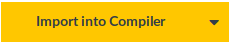
\includegraphics[height=3\fontcharht\font`\B]{images/import_compiler}}}$
 \end{enumerate}


\end{UPSTIactivite}

Import it into your mbed compiler before continuing.
Here the project tree :

\dirtree{%
 .0 /.
 .1 lib\_workshop\_2019 \DTcomment{Provided library to run the robot}.
 .2 CMPS03 \DTcomment{Compass library}.
 .2 CNY70  \DTcomment{Library for reflective sensors}.
 .2 PID    \DTcomment{Library for PID}.
 .2 Pixy   \DTcomment{Library for Pixy camera}.
 .2 VMA306 \DTcomment{Library for ultrasonic sensors}.
 .1 includes.
 .2 console\_output.h.
 .2 pin\_connexions.h \DTcomment{Declare and connect signals}.
 .2 test\_cny.h.
 .2 test\_compass.h.
 .2 test\_motor.h.
 .2 test\_us.h \DTcomment{for ultrasonic sensors}.
 .1 src.
 .2 test\_cny \DTcomment{function files to use cny70 sensors}.
 .2 test\_compass \DTcomment{function files to use compass sensor}.
 .2 test\_motor \DTcomment{function files to run motors}.
 .2 test\_us \DTcomment{function files to use ultrasonic sensors}.
 .2 console\_output.cpp \DTcomment{function to print messages to pc.}.
 .1 main.cpp.
}

The main file run an infinite loop asking the user which test does he want to run and calling the associated function.

\section{First connection}
The project you've been given is incomplete. In order for it to compile, you'll have to declare and attach a serial connexion to your pc.

The \textit{mbed} library provided by \mintinline{C}{"include "mbed.h"} defines the type \mintinline{C}{Serial} to declare a Serial connexion.

\begin{UPSTIactivite}[][Configure and connect the robot][][][To do]
 First, we need to declare and connect the serial port to communicate with the computer. Let's check the pin map to get the pin numbers we need to connect :
 \begin{center}
  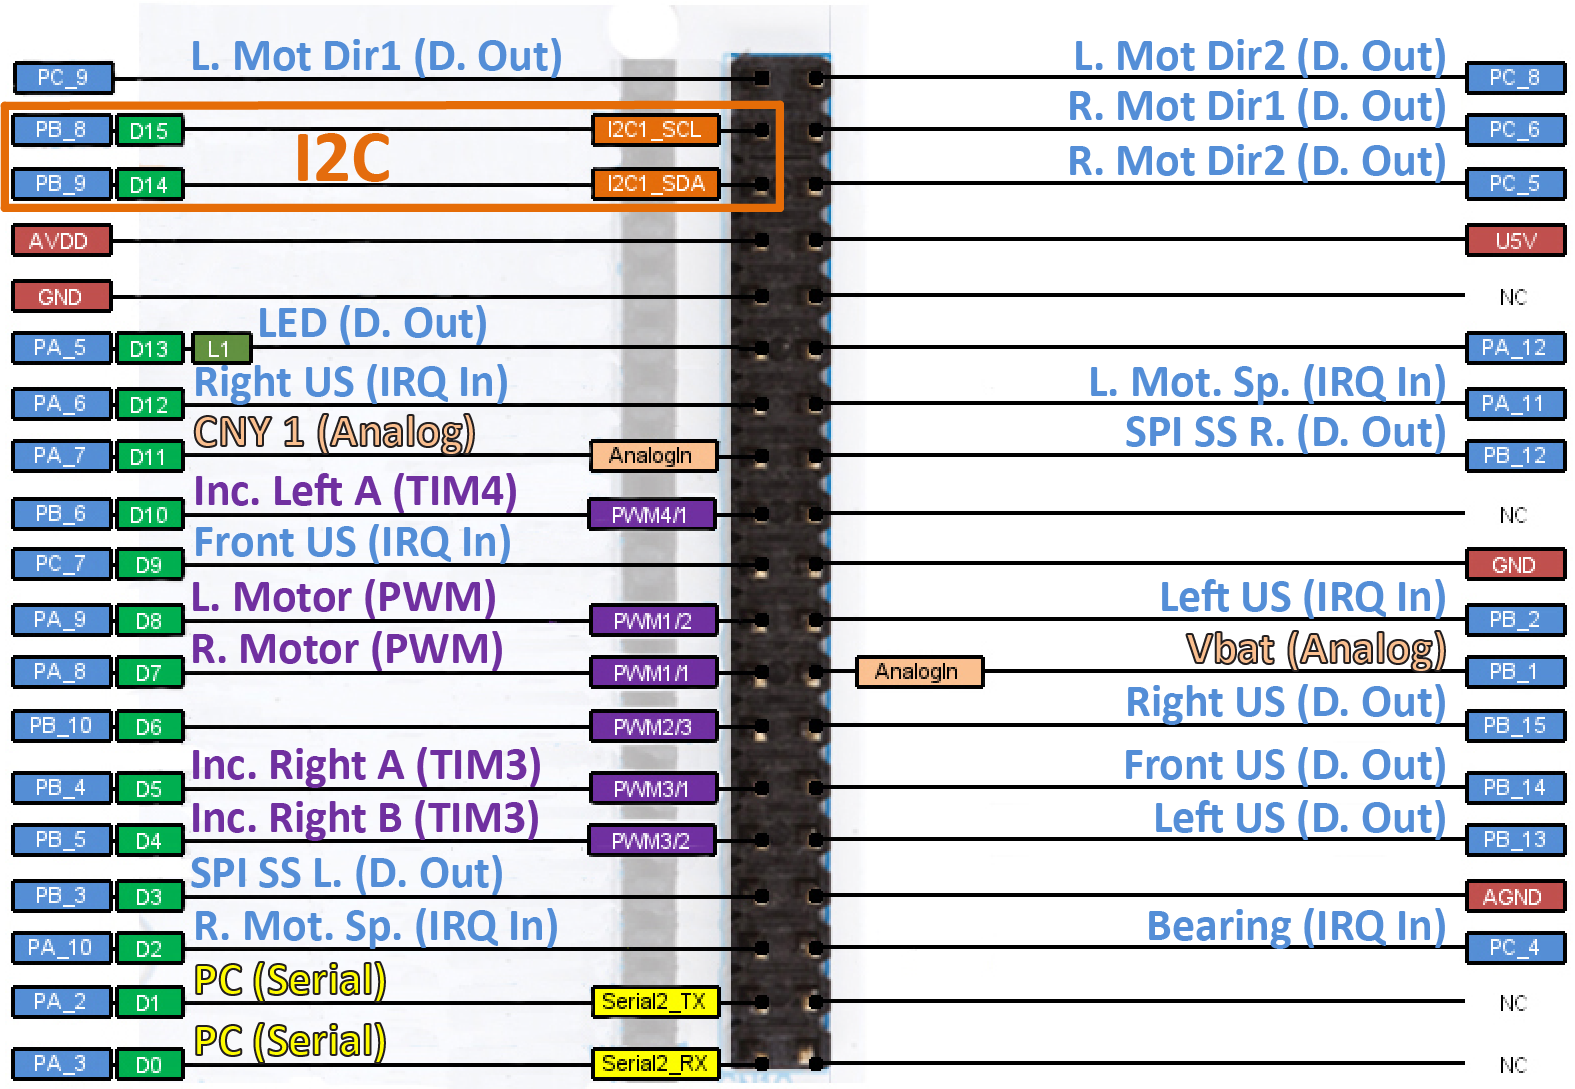
\includegraphics[viewport=0 0 190 30,height=6\fontcharht\font`\B,clip]{images/right_connectors}
 \end{center}
 \begin{enumerate}
  \item Open the file \mintinline{C}{includes/pin_connexions.h}
  \item Insert the following instruction \textbf{on line 25} in order to declare and connect the Serial port to Pins  \mintinline{C}{PA_2 and PA_3}. \mint{C}{Serial      pc      (PA_2, PA_3, 115200);}
  \item Click on the \textit{compile} button : 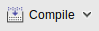
\includegraphics[height=3\fontcharht\font`\B]{images/compile_button}
  \item Save the created executable on your computer.
  \item Connect the alimentation cables (red and black wires) to the robot and switch it on.
  \item Connect the USB cable to the computer and the NUCLEO card.
        \begin{itemize}
         \item The computer should detect the card and display it as a storage device.
        \end{itemize}
  \item Copy the executable to the card (drag and drop)
  \item Open a serial communication software on your computer
        \begin{enumerate}
         \item Open Teraterm software (You'll find it on your desktop)
         \item Choose Serial Connexion
         \item Change the port to STMicroelectronics Virtual Port and hit Ok
         \item In Setup -> Serial Port, change the baud rate to \num{115200}.
        \end{enumerate}
  \item Hit the RESET button (black) on the card
 \end{enumerate}
\end{UPSTIactivite}

\pagebreak
\section{CNY 70}
\subsection{The sensor}

\begin{figure}[!ht]
 \centering
 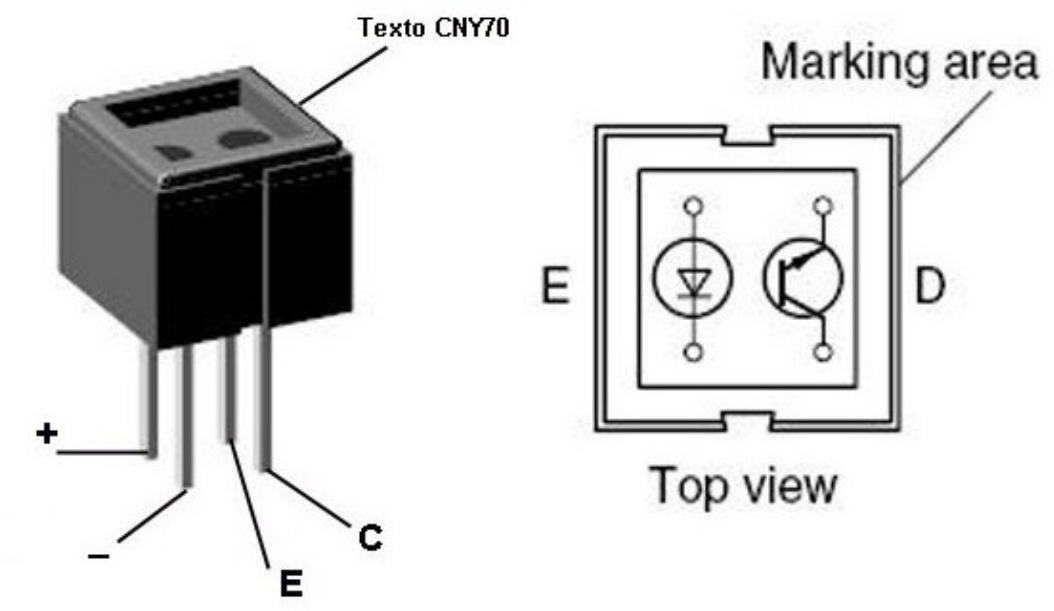
\includegraphics[width=.5\textwidth]{images/cny70}
 \caption{CNY 70}
 \label{fig:cny70}
\end{figure}

The CNY70 is a reflective optical sensor.
The emitter and the detector both use resistors to be polarized.
There is no clear formula for the detector as coupling factor varies with distance to the ground. Hence, we use trimmers to polarize the detector. 
Efficiency is a bit better with a polarization in the collector of the detector than in the emitter.

The CNY70 sensor make its detector current going up when the detector receive a light signal. To get a measure of this current, we use the voltage on the transistor's collector as shown on Figure~\ref{fig:cny70}.

\begin{figure}[!ht]
 \centering
 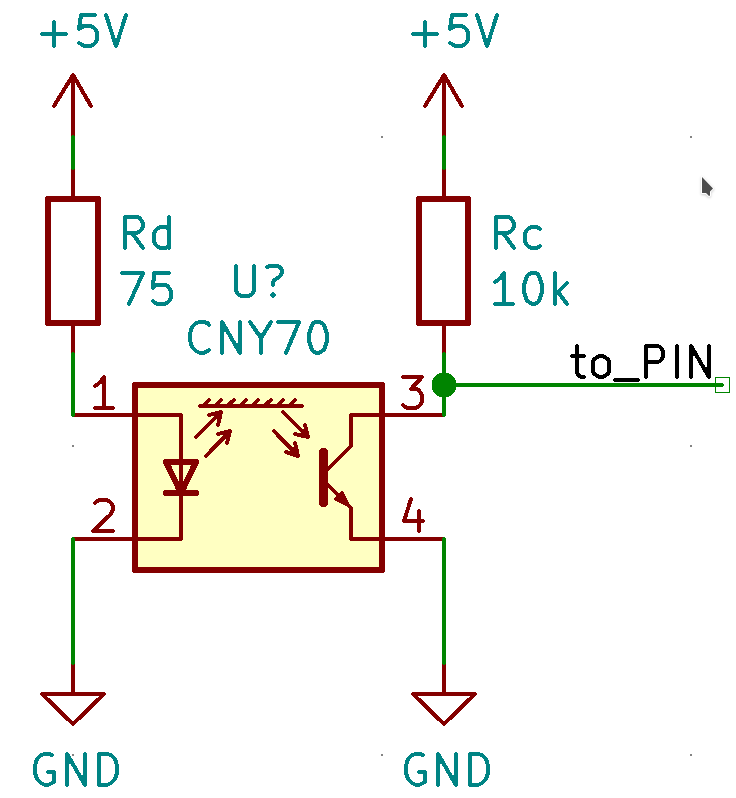
\includegraphics[width=.5\textwidth]{images/montage_cny}
 \caption{CNY 70 on the robot}
 \label{fig:cny70}
\end{figure}

\UPSTIremarque{When the detector is on a dark surface, the voltage \textit{to\_PIN} is \SI{5}{V}. \\
 When the detector is on a white surface, the voltage \textit{to\_PIN} is low t(around \SI{0}{V}).}

\subsection{Testing the CNY70 on the robot}

First, we need to identify the PIN linked to each sensor. The three sensors are connected on pins \textbf{PA\_7}, \textbf{PC\_2} and \textbf{PC\_3}.
Since we need to measure the voltage on each pin, they need to be configured as Analog inputs.

\inputminted[firstline=44, lastline=53]{C}{programmes/main.cpp}


\begin{UPSTIactivite}[][Get the CNY70 voltage][][][To do]
 \begin{enumerate}
  \item Edit the \mintinline{C}{includes/pin_connexions.h} file to \textbf{declare the sensors:}
        \begin{itemize}
         \item \mintinline{C}{cny_1} has already been declared : \mintinline{C}{DigitalIn cny_1 (PA_7);}
         \item Declare and connect \mintinline{C}{cny_2} to \textbf{PC\_2}
         \item Declare and connect \mintinline{C}{cny_3} to  \textbf{PC\_3}
        \end{itemize}
  \item Edit the \mintinline{C}{main.cpp} file to match the above code.
  \item Implement the function \mintinline{C}{ft_print_cny_analog_voltage(AnalogIn &analof_input, Serial pc)} in file \mintinline{C}{src/test_cny/ft_print_value_cny.cpp} :
        \begin{enumerate}
         \item Declare \mintinline{C}{value} and \mintinline{C}{voltage} variables (\mintinline{C}{double})
         \item Use the function \mintinline{C}{analog_input.read()} to get the converted analog value of the \mintinline{C}{analog_input} signal, put it in \mintinline{C}{value}.
         \item compute \mintinline{C}{voltage =  value * max_voltage;} to convert it.
         \item Use the \mintinline{C}{pc.printf("Voltage value : %lf ", voltage);} function to display the voltage value.
        \end{enumerate}
  \item Compile, download and transfer the executable file into the card.
  \item Identifie which sensor is connected to which signal.
        \begin{itemize}
         \item put a white sheet in front of each sensor and see which one react.
        \end{itemize}
 \end{enumerate}
\end{UPSTIactivite}


\pagebreak
\section{Controlling the motors}


Our robot moves with two DC motors.In the simplest way, the DC motor speed is proportionnal to its
input voltage $U$.
Since we want to control the motor speed, we need to control the input voltage. An efficient and quite simple way to control this voltage is using Pulse Width Modulation (PWM).


\subsection{Pulse Width Modulation}
\UPSTIdefinition{
 The duty cycle is defined as  the fraction of one period in which a signal or system is active.
}
\begin{figure}[!ht]
 \centering
 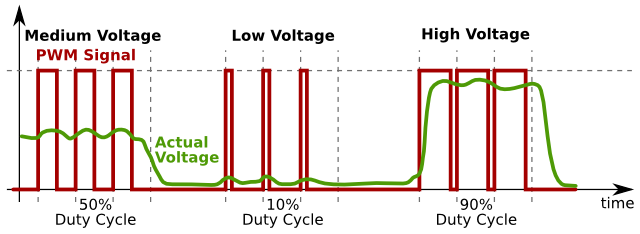
\includegraphics[width=.8\textwidth]{images/PWM_signal}
 \caption{PWM signal}
 \label{fig:PWM_signal}
\end{figure}
The idea is to make a high frequency signal and control its average value to the voltage value we want.

The higher the duty cycle is, the higher the signal average will be, as illustrated on Figure~\ref{fig:PWM_signal}.
If the duty cycle is \num{.5} (\SI{50}{\%}), the motor speed is at \SI{50}{\%} of its maximal value.

\pagebreak
\subsection{Controling the robot's motors : Full bridge}

To control the robot's motors we use a full bridge, illustrated on Figure~\ref{fig:schema_robot}.
As indicated in the table on Figure~\ref{fig:schema_robot}, \mintinline{C}{IN_1} and \mintinline{C}{IN_2} control the direction.
We control the speed by connecting the PWN to the \mintinline{C}{ENABLE} pin.

\begin{figure}[!ht]
 \centering
 \begin{subfigure}[b]{.7\textwidth}
  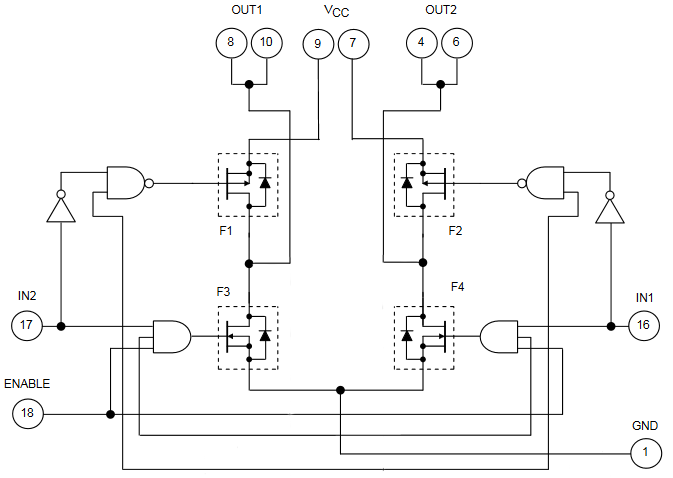
\includegraphics[width=\textwidth]{images/robot_schema}
  \caption{Schematic}
 \end{subfigure}

 \begin{subfigure}[b]{.7\textwidth}
  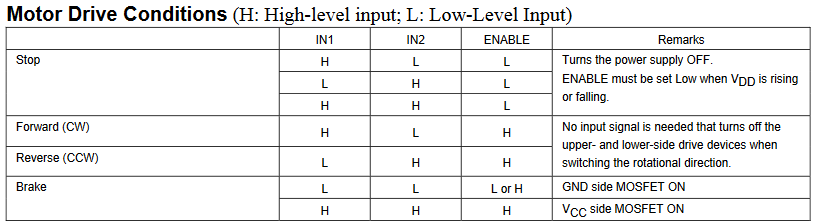
\includegraphics[width=\textwidth]{images/table_full_bridg}
  \caption{Control}
 \end{subfigure}
 \caption{Full bridge}
 \label{fig:schema_robot}
\end{figure}

\pagebreak
\subsection{Testing the motors}

For testing if the PWM controlling the motors is fully functionnal, we use the \mintinline{C}{ft_test_motor} function.
This function ask the user to define the wanted duty cycle and call the \mintinline{C}{ft_run_motor} function to run the PWM. You will implement this function to run the motors :

\inputminted[numbersep=4pt,linenos,firstline=11]{C}{programmes/ft_run_motor.cpp}
\begin{UPSTIactivite}[][Testing the motors][][][To do]
 \begin{enumerate}
  \item On the pinmap of the nucleo card (Figure~\ref{fig:right_connector} and Figure~\ref{fig:left_connector}), look for \textit{L. Mot Dir1}, \textit{L. Mot Dir2}, \textit{R. Mot Dir1} and \textit{R. Mot Dir2} and write the associated PIN.
  \item In the mbed compiler, edit the file \mintinline{C}{includes/pin_connexions.h}
        \begin{enumerate}
         \item Declare and connect the \mintinline{C}{DigitalOut} signals \mintinline{C}{DIR_1L, DIR_2L, DIR_1R, DIR_2R} to control the direction of left and right motor.
         \begin{itemize}
           \item \mintinline{Cpp}{DigitalOut DIR_1L (PC_9);}
         \end{itemize}
         \item Declare and connect the \mintinline{C}{PwmOut} signals \mintinline{C}{Pwm_ML and Pwm_MR} to control the PWM of each motor.
         \begin{itemize}
           \item \mintinline{cpp}{PwmOut Pwm_ML (PA_9);}
         \end{itemize}
        \end{enumerate}
  \item In the mbed compiler, edit the \mintinline{C}{Src/test_motor/ft_run_motor.cpp} file so that
        \begin{enumerate}
         \item Set the \mintinline{C}{dirA} and \mintinline{C}{dirB} value depending on the wanted direction,
         \item Set the PWM signal to the \mintinline{C}{duty_cycle} given in argument.
        \end{enumerate}
  \item Edit \mintinline{C}{main.cpp} to call \mintinline{C}{ft_test_motor} function:
        \inputminted[firstline=67,lastline=68]{C}{programmes/main.cpp}
        \inputminted[firstline=72,lastline=73]{C}{programmes/main.cpp}
 \end{enumerate}
\end{UPSTIactivite}


\pagebreak
\section{Testing other sensors}
\begin{UPSTIactivite}[][Testing other sensors][][][To do]
 Use the interface to test if every sensor is working.
\end{UPSTIactivite}

\subsection{VMA 306 : Ultrasonic sensor}
To use the VMA306 sensor, we set the \textit{Trig} pin to \textbf{high} for at least \SI{10}{\micro s}, then the sensor send a burst of 8 x 40KHz pulses and set the \textit{echo} pin to \textbf{high}. When the burst comes back to the sensor (caused by the echo), the sensor set its \textit{echo} pin to \textbf{low} (illustrated on Figure \ref{fig:vma306}).

\begin{figure}[!ht]
 \centering
 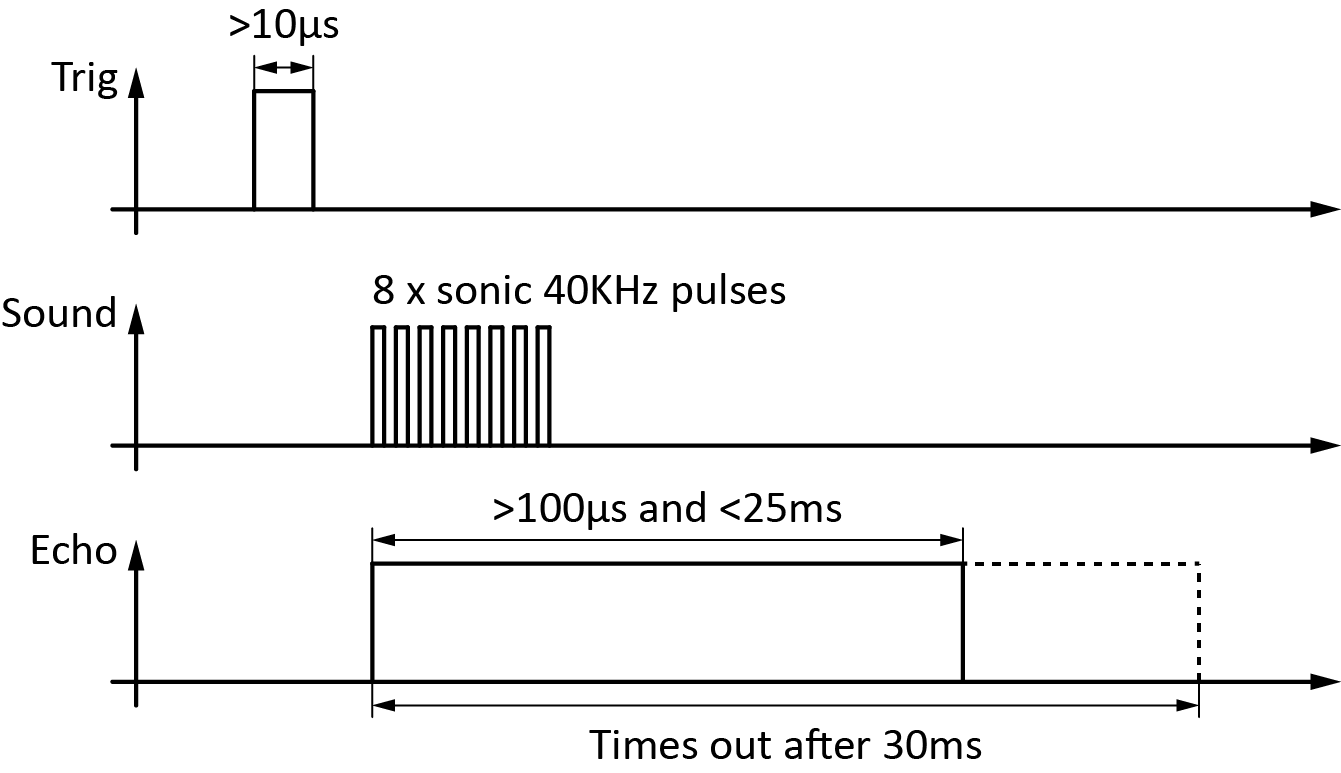
\includegraphics[width=.5\textwidth]{images/echo_vma}
 \caption{VMA306 sensor}
 \label{fig:vma306}
\end{figure}

Thus, the time during which the \textit{Echo} pin is \textbf{high} represent the time the sound traveled.
Let $t_{\text{up}}$ be the time of \textit{Echo} being \textbf{high} and $v_s = \SI{340}{m/s}$ the sound speed. The measured distance $d$ can be expressed as \[ d = v_s \times t_{\text{up}} \]



To avoid false detection each VMA306 send his pulse every 150ms and with a 50ms delay after previous one.
There are 3 VMA306 on the robot: one on the left, one on the front, one on  the right.

In the provided library, you can access to VMA306 data.

%\subsection{Compass}
%\subsubsection{The sensor}

The CMPS03 is a compass allowing us to get a bearing in order to follow a line of sight.
It provides the bearing both through an I2C bus and a PWM signal.

\paragraph{Bus I2C}
To access the I2C bus, we use \textbf{PB\_8} as \textit{SCL} and \textbf{PB\_9} as \textit{SDA}.
There are 2 ways to get the bearing through the I2C protocol:
\begin{itemize}
  \item 1-byte data bearing (0 to 255) using register 1.
  \item 2-bytes data bearing (0 to 3599) using registers 2 and 3 (auto  incrementation).
\end{itemize}

\paragraph{PWM signal}
To access the bearing through the PWM signal, one should look at the width of the pulse on the Pin 4 of the CMPS03 (connected to \textbf{PC\_4}).
The pulse width varies from \SI{1}{ms} when bearing is \SI{0}{\degree} to \SI{36.99}{ms} when bearing is \SI{359.9}{\degree}. The signal goes low for 65ms between pulses.


\section{Pin map of the robots}
\begin{figure}
 \centering
 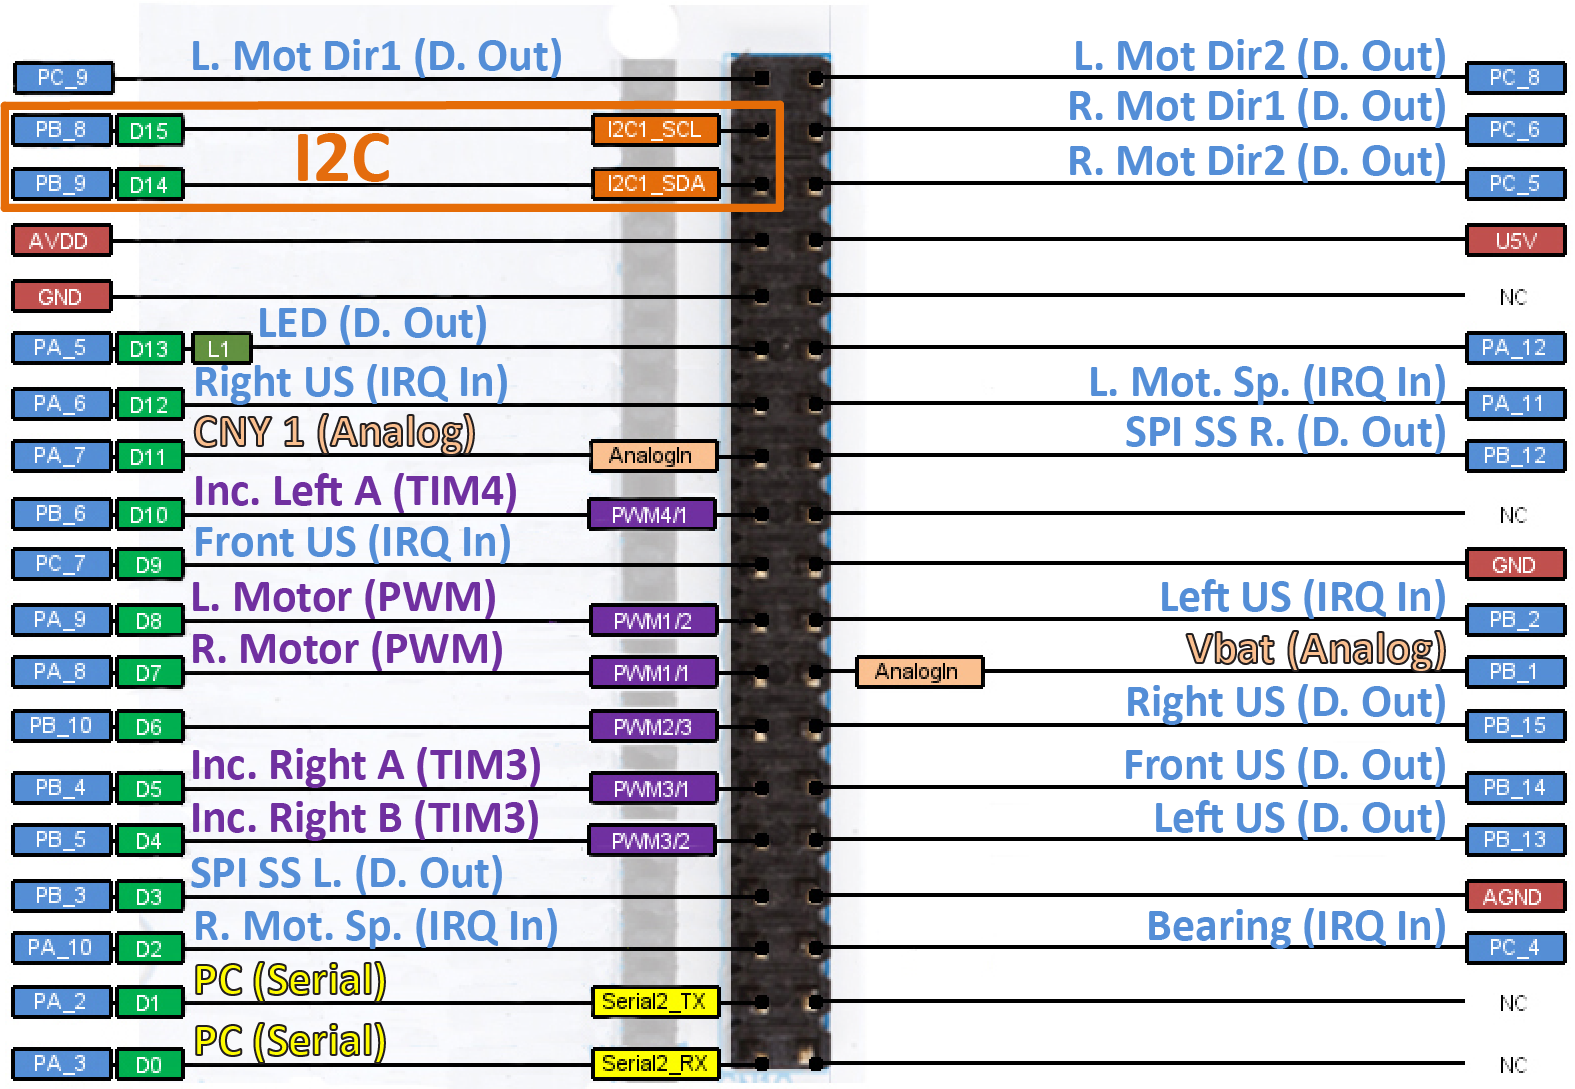
\includegraphics[width=\textwidth]{images/right_connectors}
 \caption{PIN map of the right connector}
 \label{fig:right_connector}
\end{figure}

\begin{figure}
 \centering
 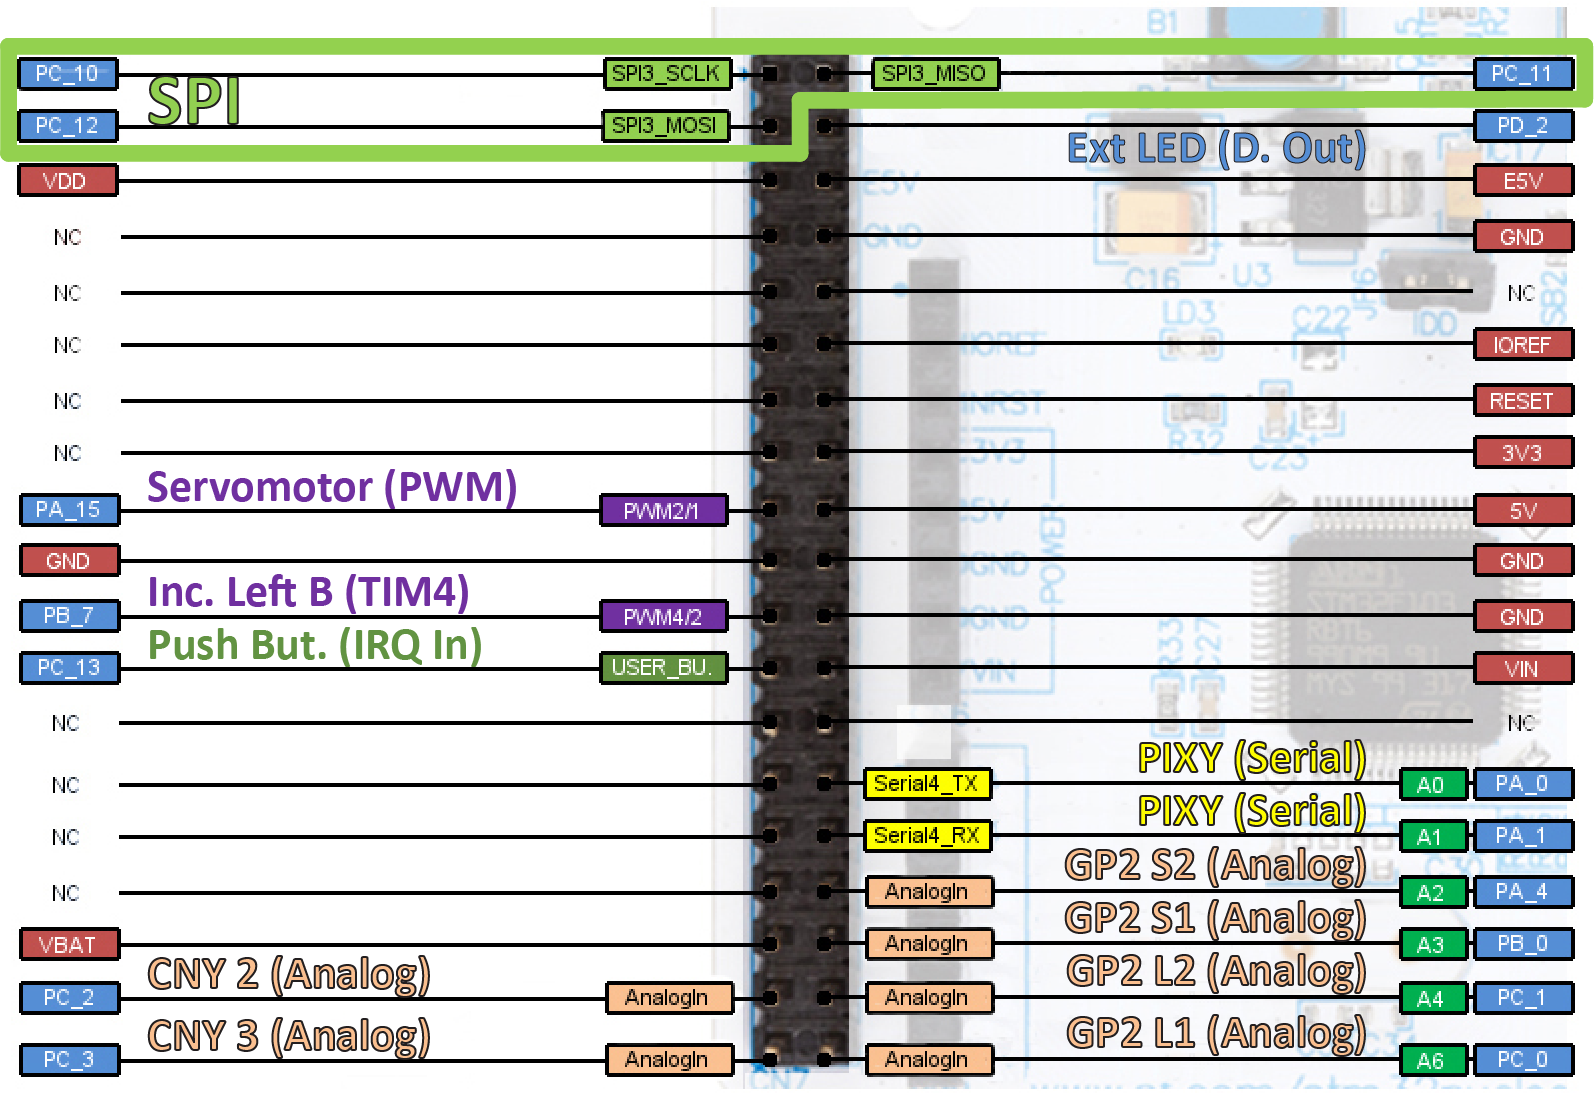
\includegraphics[width=\textwidth]{images/left_connector}
 \caption{PIN map of the left connector}
 \label{fig:left_connector}
\end{figure}
\end{document}
